\chapter{Method}
\label{sec:method}

\section{Data Preparation}
Data preparation is a critical phase in the modeling process, especially for a task involving complex and diverse datasets like ours. Our data preparation process is designed to ensure that the data fed into the model is clean, structured, and suitable for effective analysis and modeling. The following sections describe the steps taken to prepare the data for the multimodal product classification task.

\subsection{Loading and Initial Cleaning}

The first step involves loading the training data from CSV files.  We ensure that any missing values are handled appropriately by filling them with empty strings. This step is crucial to maintain consistency in the dataset.

\subsection{Text Data Preprocessing}

For the 'designation' and 'description' columns, we apply a custom text processing function. This function limits the length of text data to the first 70 tokens, ensuring consistency and manageability in text length. This is also done because a CLIP (Contrastive Language–Image Pretraining) model is used, which can only process up to 76 tokens. Because the data is then preprocessed by the CLIP model, we do not perform any further text preprocessing.

\subsection{Categorical Encoding of Labels}

In our multimodal product classification task, the target variable 'prdtypecode' represents the category to which each product belongs. This variable is inherently categorical, meaning it represents discrete, non-numeric categories. Each unique 'prdtypecode' corresponds to a different type of product.

Categorical Encoding is used because each ‘prdtypecode’ is a distinct category with no inherent numerical relationship or order between them. Categorical encoding ensures that the model treats these categories as separate and distinct without assuming any numerical relationship or hierarchy among them \cite{potdar-2017}. If left as is, the model might misinterpret the categorical codes as ordinal or interval  data, leading to incorrect assumptions about the proximity or similarity between different categories.

For this use case One-Hot encoding was used. It converts the categorical target variable into a binary matrix. In this matrix, each category is represented by a vector where only one element is '1', and the rest are '0' \cite{cerda-2018}. This representation avoids any notion of order or magnitude among categories, which is essential for unbiased classification.
With one-hot encoding, no category is given undue preference. For instance, if numeric labels were used directly, the model might assume that higher numbers have more significance or weight, which is not the case in categorical classification.
While one-hot encoding is beneficial, it does increase the dimensionality of the dataset. Each unique category becomes a new feature in the dataset. In cases with many categories, this can lead to a large increase in the number of input features, potentially causing issues like the "curse of dimensionality"\cite{altman-2018}. However, in our context, the benefits of clear and distinct categorical representation outweigh these concerns.

\section{Visualisation}

\section{Feature Extraction}

While data preparation sets the stage for clean and structured input, feature extraction is where the true essence of the data is captured, turning raw information into a form that can be understood by the multimodal classification model. This chapter will delve into the methods employed to extract features from images and text, leveraging the power of OpenAI's CLIP model, and detail the subsequent steps that prepare these features for classification.

\subsection{Integrating CLIP for Enhanced Multimodal Product Classification}
Central to our approach is the integration of OpenAI's CLIP (Contrastive Language–Image Pretraining) model. CLIP is a foundation model based on a transformers and Vit architecture to extract text and image features in the same embedding space.


\begin{figure}[H]
    \centering
    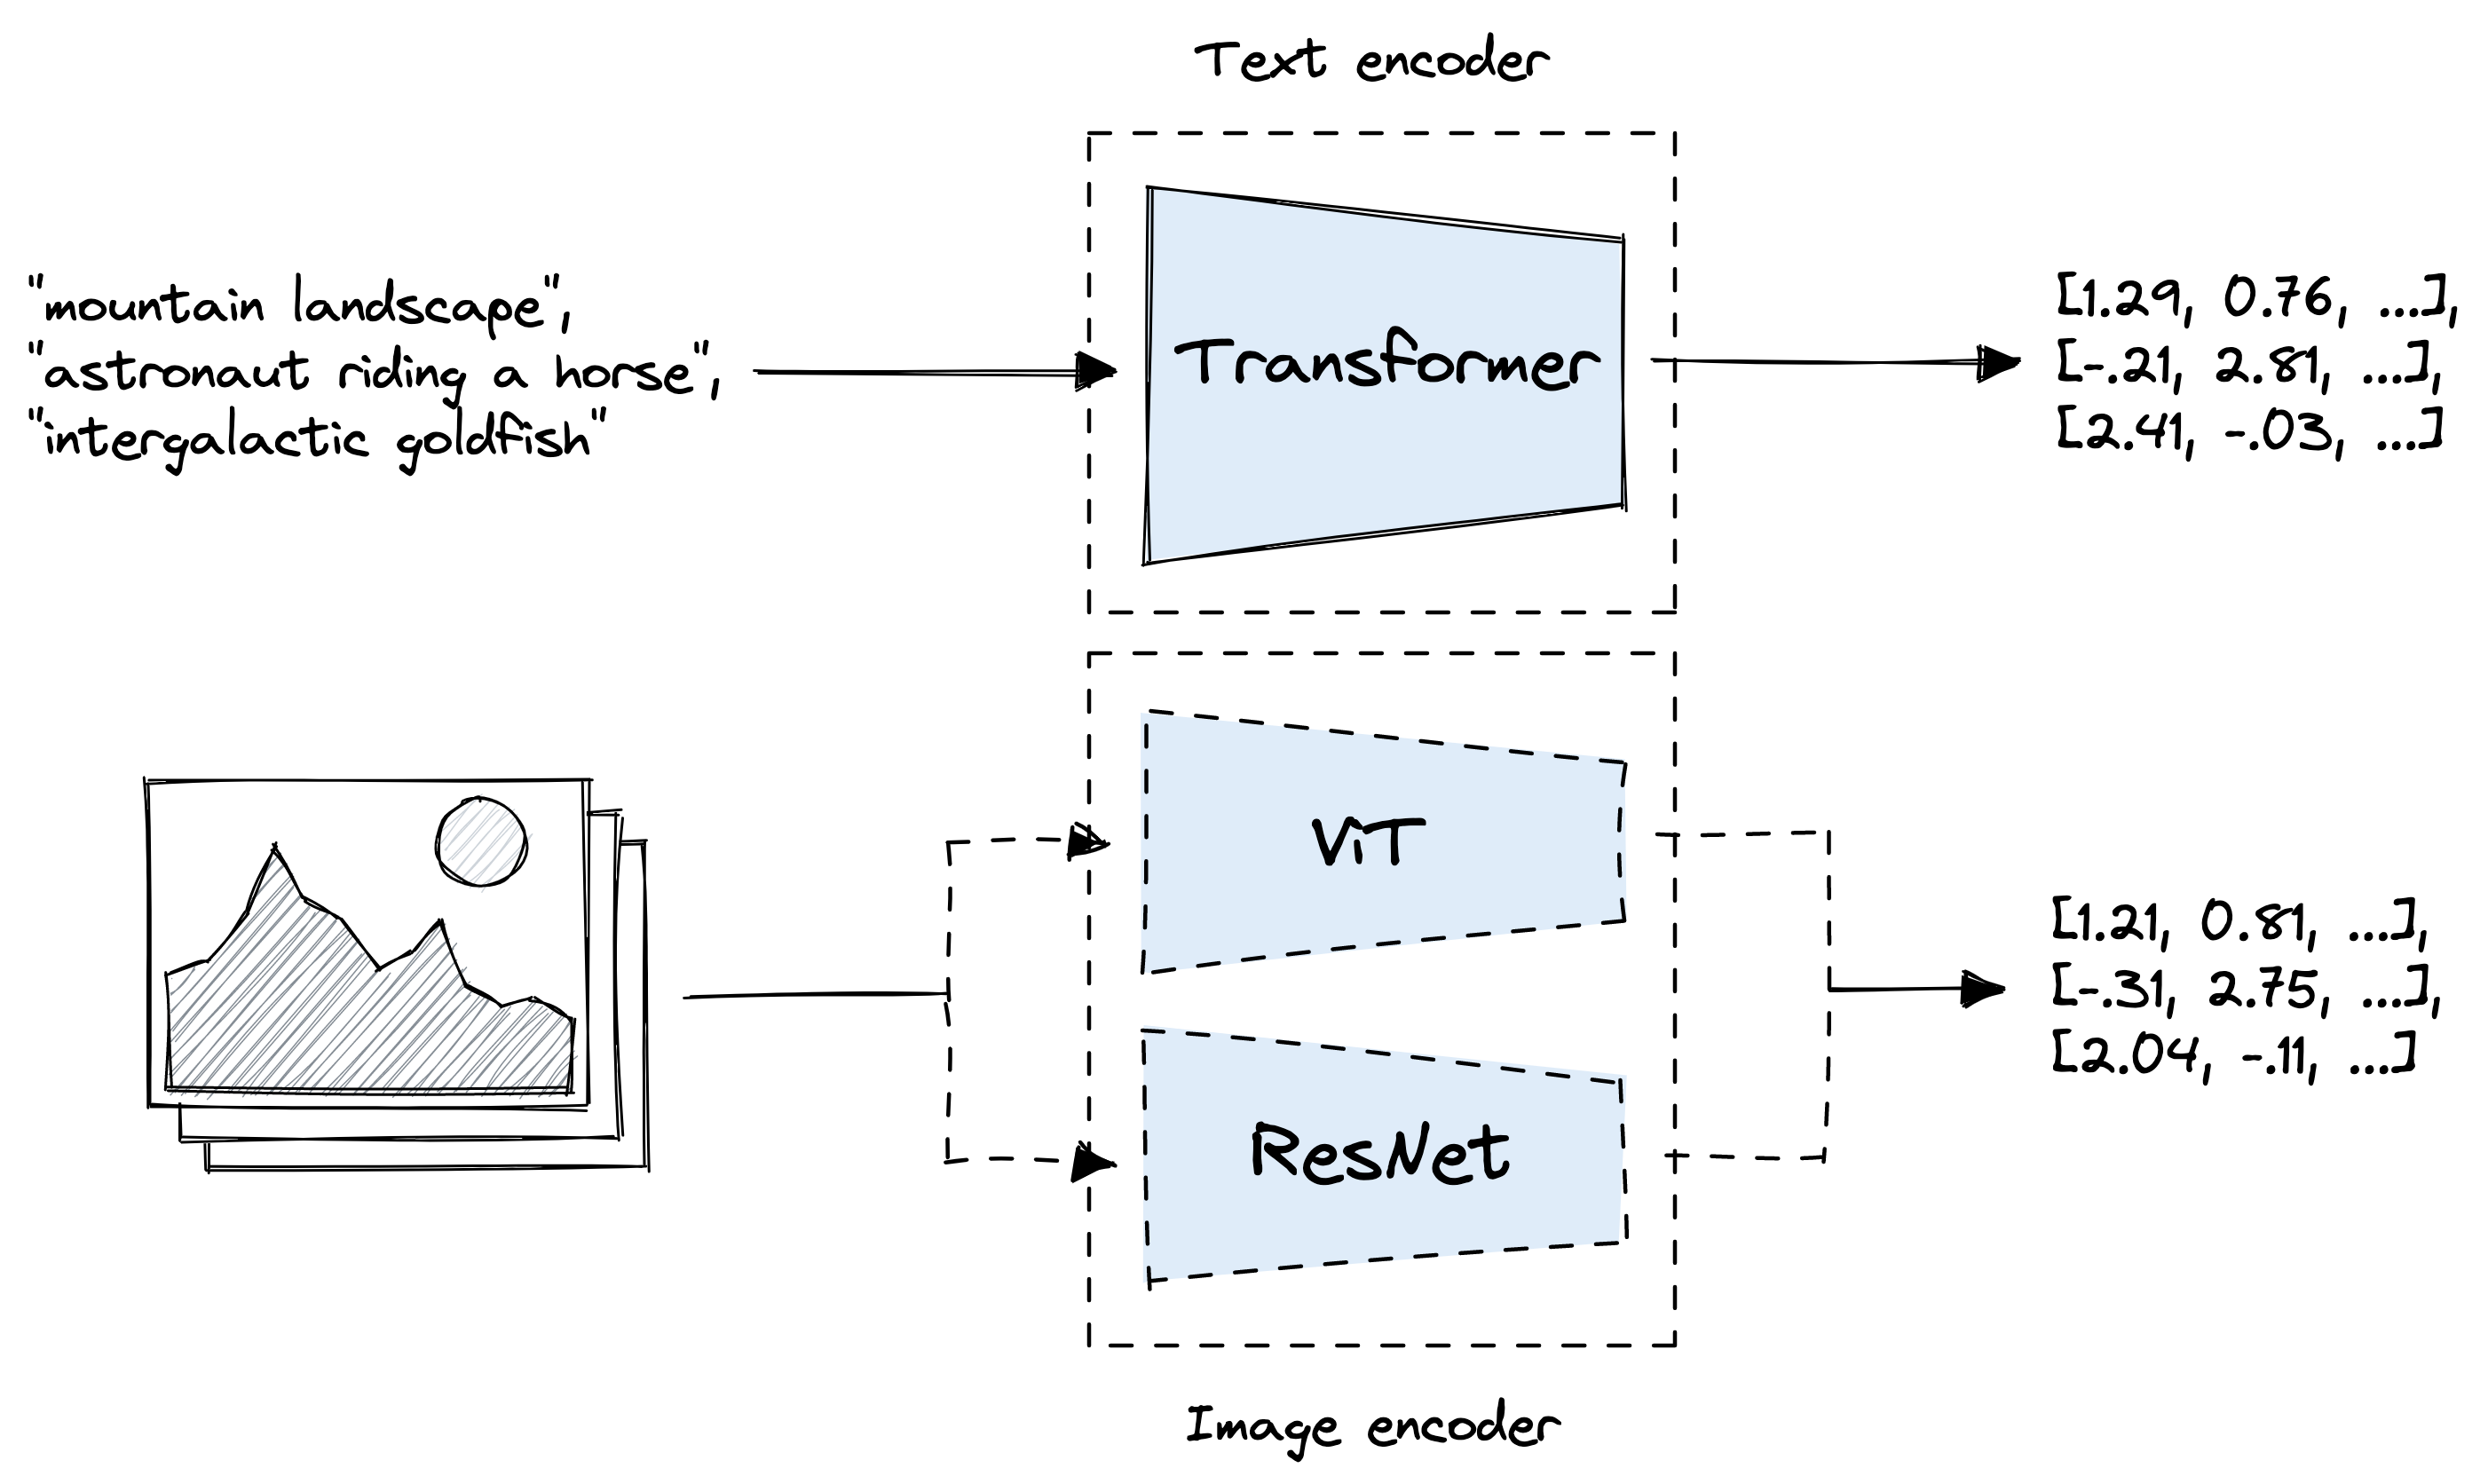
\includegraphics[width=\textwidth]{clip_description.png}
    \caption{Clip Model presentation \\ source: pinecone.io}
    \label{fig:clip-architecture}
\end{figure}


As can be seen in the figure \ref{fig:clip-architecture}, CLIP operates on a dual-encoder structure, comprising an image encoder and a text encoder. This architecture is instrumental in processing and correlating visual and textual inputs. The model's training utilizes a contrastive learning method, where it is exposed to numerous images and their corresponding textual descriptions, drawing from a diverse and extensive internet-sourced dataset. This training enables CLIP to develop a nuanced understanding of the intricate relationships between text and images \cite{radford-2021}.
We are going to use the Clip Model, hoping that the feature extraction done by the clip encoder will provide embeddings that will be separable by the classifier.

\begin{figure}[H]
    \centering
    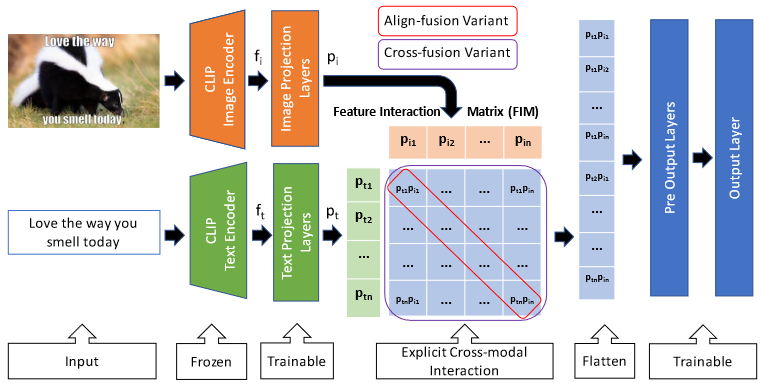
\includegraphics[width=\textwidth]{hateclip}
    \caption{Proposed architecture of Hate-CLIPper for Multimodal Hateful Meme Classification \cite{radford-2021}}
    \label{fig:architecture}
\end{figure}

In the realm of product classification, CLIP's integration offers a transformative potential. Our model leverages CLIP's proficiency in associating product images with their textual descriptions, such as titles and detailed narratives. This synergy allows for a more nuanced and accurate classification of products into their respective categories.

Using CLIP's pre-trained encoders allows for the leveraging of a knowledge base that the model has learned from a wide array of internet data, which we otherwise couldn't capture.

\subsection{Feature Interaction Matrix}
The Feature Interaction Matrix (FIM) (As seen in Figure \ref{fig:architecture}) stands at the forefront of our feature extraction process, embodying a sophisticated mathematical framework that captures the non-linear relationships between textual and visual features. This matrix is constructed by an outer product operation between feature vectors obtained from CLIP’s image and text encoders, resulting in a rich representation that encapsulates the complex interplay between the two modalities. Unlike simple concatenation methods, which may merely stack features without considering their interdependence, the FIM delves deeper into the nuanced dynamics of cross-modal interactions. By explicitly modeling these interactions, the FIM facilitates the learning of conjunctional patterns and co-dependencies that are often critical for understanding multimodal content. The approach, as detailed in the "Hate-CLIPper" paper, leverages the inherent strengths of CLIP’s robust feature extraction, while extending its capabilities to discern the intricate associations that simpler models might overlook. The FIM thereby enables a more holistic and contextually aware representation of the data, enhancing the model's ability to perform accurate classification in complex multimodal tasks.

\section{Modelling}
asdad

